%! suppress = NonBreakingSpace
%! BibTeX Compiler = biber

% Preamble
\documentclass[12pt]{article}
\renewcommand{\baselinestretch}{1.5}
\author{Christoph Derszteler}

% Packages
\usepackage[
  left=4cm,
  right=3cm,
  top=3cm,
  bottom=3cm
]{geometry}
\usepackage[bottom]{footmisc}
\usepackage[utf8]{inputenc}
\usepackage[T1]{fontenc}
\usepackage[german]{babel}
\usepackage{blindtext}
\usepackage{float}

\usepackage{hyperref}
\hypersetup{
  linkcolor=black,
  linktoc=all,
}

\usepackage[
  citestyle=alphabetic,
  bibstyle=alphabetic,
]{biblatex}
\DeclareCiteCommand{\footcite}[\mkbibfootnote]
{\usebibmacro{prenote}}
{\usebibmacro{citeindex}%
\printtext[brackets]{\usebibmacro{cite}}}
{\multicitedelim}
{\usebibmacro{postnote}}
\addbibresource{sources.bib}

\usepackage{graphicx}
\usepackage{booktabs}
\usepackage{siunitx}
\usepackage{amsfonts}
\usepackage{amsmath}
\usepackage{amssymb}
\usepackage{xcolor}
\usepackage{tikz}

\counterwithin*{equation}{section}
\counterwithin*{figure}{section}
\renewcommand{\theequation}{\arabic{section}.\arabic{equation}}
\renewcommand{\thefigure}{\arabic{section}.\arabic{figure}}
\renewcommand{\thetable}{\arabic{section}.\arabic{table}}

\usepackage{tocloft}
\renewcommand{\cftpartleader}{\cftdotfill{\cftdotsep}}
\renewcommand{\cftsecleader}{\cftdotfill{\cftdotsep}}

\newcommand{\sectiontitle}{}
\newcommand{\newsection}[2]{\renewcommand{\sectiontitle}{#1}\section{#1}\label{sec:#2}}

\usepackage{fancyhdr}
\fancypagestyle{table-of-contents}{
  \fancyhead{}
  \rhead{\thepage}
  \chead{INHALTSVERZEICHNIS}
  \fancyfoot{}
  \renewcommand{\headrulewidth}{0.4pt}
}
\pagestyle{fancy}
\lhead{\thesubsection}
\chead{\MakeUppercase{\sectiontitle}}
\rhead{\thepage}
\fancyfoot{}
\renewcommand{\headrulewidth}{0.4pt}

% Document
\begin{document}
  \begin{titlepage}
  \begin{center}
    \vspace{1cm}

    Heinrich-Böll-Gymnasium Troisdorf\\
    Schuljahr 2022/2023

    \vspace{1cm}
    \Huge
    \line(1,0){400}\\
    \textbf{Die mathematischen Grundlagen der Mandelbrot-Menge}\\
    \line(1,0){300}\\

    \vspace{0.75cm}
    \Large
    und deren visuelle Darstellung mithilfe von Computerprogrammen

    \vspace{2cm}
    \large
    verfasst von\\
    \Large
    \textbf{Christoph Derszteler}

    \vfill
    \large
    Leistungskurs Mathematik\\
    Betreuer: Frau Dammers\\
    Abgabetermin: 23.02.2022 12:00 Uhr CET\\
  \end{center}
\end{titlepage}
  \newpage

  \tableofcontents{\thispagestyle{table-of-contents}}

  \newsection{Einleitung}{introduction}

Die Mandelbrot-Menge ist durch ihre hübschen, ansehnlichen Darstellungen verglichen
mit anderen mathematischen Phänomenen recht bekannt.
Dies liegt jedoch nicht nur an ihrer rein visuellen Attraktivität,
sondern vielmehr auch an Benoît Mandelbrot\hyperref[app:3]{[A.3]},
dem Entdecker dieser Menge.
Dieser sorgte mit seinen vielen Vorträgen und Büchern dafür, dass sich Fraktale,
also selbstähnliche\footnote{
  Das heißt, sich selbst wiederholend oder in ähnlicher Form erneut aufkommend.
}, geometrische Figuren mit gebrochener Dimension\footnote{
  Im Vergleich zu zum Beispiel einem zwei-dimensionalen Viereck.
}, vornehmlich die Mandelbrot-Menge, in der Bevölkerung weit verbreiteten
~\footcite[Vgl. letzten Absatz]{ibm_fractal_2011}.

Obwohl die Natur mit ihren fraktal-ähnlichen Formationen wie dem Aufbau einer
Schneeflocke, dem Verlauf eines Flusses oder die Verteilung von Baumästen
~\cite{nnart_fractals_nodate} die Inspiration für Mandelbrot war
~\cite{zink_kosmische_2014}, so liegt der Ursprung dieser Arbeit in den für
manchen simpler erscheinenden, viel moderneren aber dennoch genauso spannenden,
computer-generierten Videos\footcite[Vgl. bspw.][]{maths_town_eye_2017},
die man im Internet finden kann.
Mit unter anderem der Frage, wie diese Videos in Ansätzen generiert werden können
und vielem weiteren beschäftigt sich diese Arbeit.

Dafür jedoch und zum vollen Verständnis der Mandelbrot-Menge ist Grundlagenwissen
gewisser Themengebiete erforderlich, das in Kapitel 2 näher erörtert wird.
Kapitel 3 beschäftigt sich daraufhin mit der Mandelbrot-Menge selbst und insbesondere
mit der Analyse visueller Darstellungen dieser.
Abschließend befasst sich diese Arbeit in Kapitel 4 mit der praktischen Anwendung
der Mandelbrot-Menge in Form von Bildgenerierungen mithilfe von Computern als auch
anderweitigen Zusammenhänge zwischen dem theoretischen, mathematischen Konzept
der Mandelbrot-Menge und der realen Welt.

  \newsection{Benötiges Vorwissen}{prior-knowledge}

Dieses Kapitel befasst sich mit den ben\"otigten mathematischen Grundlagen, um
der restlichen Arbeit beziehungsweise der weiteren Ausführung der Mandelbrot-Menge
selbst folgen zu k\"onnen.
Daf\"ur wird zun\"achst das Konzept der komplexen Zahlen als auch der f\"ur den weiteren
Verlauf ben\"otigter Umgang mit diesen er\"ortert.
Darauffolgend soll lediglich das Prinzip und die Eigenschaften von Iterationen grob
anhand zweier Beispiele skizziert werden.

\subsection{Komplexe Zahlen}\label{subsec:complex-numbers}

Unter den komplexen Zahlen $\mathbb{C}$ versteht man die nächst größere Zahlenmenge
nach den reellen Zahlen $\mathbb{R}$,
die zus\"atzlich zu einem Realteil auch einen sogenannten Imagin\"arteil besitzen.
Sie werden im weiteren Verlauf in der kartesischen Form
$z = a + bi$ dargestellt, wobei $a$ der Realteil und $bi$ der Imagin\"arteil ist.
Der Buchstabe $i$ steht hierbei für die imaginäre Einheit und
ist definiert durch die Gleichung $i^2 = -1$.

\subsubsection{Multiplikation \& Addition von komplexen Zahlen}
\label{subsubsec:addition-and-multiplication-of-complex-numbers}

Viele Rechenoperationen mit komplexen Zahlen funktionieren anders, als man sie
von den reellen oder natürlichen Zahlen gewohnt ist.
Im Folgenden werden zwei dieser unterschiedlich funktionierenden
Operationen vorgestellt:

Zur Addition zwei komplexer Zahlen addiert man den
Realteil und den Imagin\"arteil getrennt voneinander und fügt diesen
danach wieder zusammen~\cite[S. 2]{lichtenegger_komplexe_2002}:
$(a_1 + {b_1}i) + (a_2 + {b_2}i) = a_1 + a_2 + (b_1 + b_2)i$.

Um komplexe Zahlen zu multiplizieren, wendet man das Distributivgesetz an,
indem man den zweiten Faktor ebenfalls in seinen Realteil und seinen
Imagin\"arteil trennt und diese jeweils einzeln mit dem ersten Faktor multipliziert
\cite[S. 2f.]{lichtenegger_komplexe_2002}.
Die zwei entstehenden Produkte lassen sich dann wie oben beschrieben addieren.
Bei der Multiplikation mit dem Imagin\"arteil multipliziert man unter anderem
zwei imagin\"are Elemente miteinander.
Da $i^2 = -1$ gilt, entsteht durch diese Multiplikation
ein negatives, aber reales Produkt.
Wie in \hyperref[app:2]{A.2} gezeigt, gilt somit:
$ (a + bi)(c + di) = ac - bd + (bc + ad)i $

Das in der Mandelbrot-Menge häufig angewandte Quadrieren von komplexen Zahlen,
lässt sich mit der kartesischen Form ebenfalls herleiten \hyperref[app:3]{[A.3]}.
Für eine gegeben, zu quadrierende, komplexe Zahl $a + bi$ gilt somit:
$(a + bi)^2 = a^2 - b^2 + 2abi$


Ein illustriertes Beispiel soll beide Rechenoperationen veranschaulichen:

\begin{equation}\label{eq:complex-numbers-example}
  \begin{split}
    (\begingroup\color{red} -3\endgroup + \begingroup\color{blue} 6i\endgroup)^2
      + (\begingroup\color{red} 7\endgroup + \begingroup\color{blue} (-4i)\endgroup) \\
    = (
        (\begingroup\color{red} -3\endgroup \cdot \begingroup\color{red} (-3)\endgroup)
          - (\begingroup\color{red} 6\endgroup \cdot \begingroup\color{red} 6\endgroup)
        + (
          (\begingroup\color{blue} 6\endgroup \cdot \begingroup\color{blue} (-3)\endgroup)
          + (\begingroup\color{blue} -3\endgroup \cdot \begingroup\color{blue} 6\endgroup)
        )i
      )
      + (\begingroup\color{red} 7\endgroup + \begingroup\color{blue} (-4i)\endgroup) \\
    = (\begingroup\color{red} -27\endgroup + \begingroup\color{blue} (-36i)\endgroup)
      + (\begingroup\color{red} 7\endgroup + \begingroup\color{blue} (-4i)\endgroup) \\
    = \begingroup\color{red} -20\endgroup + \begingroup\color{blue} (-40i)\endgroup
  \end{split}
\end{equation}

\subsubsection{Graphische Darstellung komplexer Zahlen}

Komplexe Zahlen können wie auch Zahlen anderer Zahlenmengen grafisch
dargestellt werden.
Da komplexe Zahlen jedoch sowohl aus einem Realteil und einem Imagin\"arteil
bestehen, reicht eine Achse nicht aus, um diese darzustellen;
stattdessen braucht man eine Ebene\footnote{
  Ebenfalls unter komplexer Zahlenebene und gaußsche Zahlenebene zu finden.
}.
Diese komplexe Zahlenebene teilt den Realteil auf die waagerechte Achse und
den Imagin\"arteil auf die horizontale Achse auf.
Eine komplexe Zahl $z = a + bi$ besitzt somit die Koordinaten $ P(a|b)$.


Eine komplexe Zahl lässt sich wie auch eine reelle Zahl absolut betrachten, wobei
dieser absolute Wert ebenfalls als einen Abstand zum Ursprung zu betrachten ist
\cite[S. 3]{lichtenegger_komplexe_2002}.
Aufgrund dessen, dass eine komplexe Zahl aus zwei Komponenten besteht, lässt sich
der Abstand über den Satz des Pythagoras berechnen:

\begin{equation}\label{eq:absolute-complex-number}
  |z|^2 = a^2 + b^2
  \quad
  \text{ beziehungsweise }
  \quad
  z = \sqrt{a^2 + b^2}
\end{equation}

\begin{figure}[H]
  \centering
  \begin{tikzpicture}
    \begin{scope}[thick,font=\scriptsize]
      \draw (0,0) -- (0,2);
      \draw (2,0) -- (2,3);
      \draw (0,0) -- (2,3);
      \fill[fill=gray!15] (0,0)--(2, 0)--(2,3);
      \node at (1,0.25) {$ a $};
      \node at (2.25,1.5) {$ b $};
      \node at (0.70,1.5) {$ |z| $};

      \draw [fill=black] (2,3) circle(0.05);
      \draw [fill=black] (-3.4, -1.75) circle(0.05);
      \node at (2.75,3.25) {$ P_1(2|3i)$};
      \node at (-2,-1.50) {$ P_2(-3.4|-1.75i)$};

      \draw [->] (-4,0) -- (4,0) node [above left]  {$Re$};
      \draw [->] (0,-4) -- (0,4) node [below right] {$Im$};

      \foreach \n in {-3,...,-1,1,2,...,3}{
        \draw (\n, 3pt) -- (\n, -3pt)   node [below] {$\n$};
        \draw (3pt,\n) -- (-3pt,\n)   node [left] {$\n i$};
      }
    \end{scope}
  \end{tikzpicture}
  \caption{
    Komplexe Ebene mit den Punkten $ P_1, \text{ und } P_2$
    und dem absoluten Wert $|z| \text{ vom Punkt } P_1$.
  }
  \label{fig:complex-numbers-figure-example}
\end{figure}
\subsection{Iterationen}\label{subsec:iterations}

Iterationen beziehen sich in der Mathematik auf das Wiederholen einer bestimmten
Prozedur beziehungsweise in diesem Fall einer Berechnung.
Bei Funktionsiterationen iteriert (also wiederholt) man die Berechnung eines
Funktionswerts mit dem Funktionsargument des vorherigen Funktionswerts:
$z_1 = f(z_0),\, z_2 = f(z_1),\, z_3 = f(z_2),\, \cdots,\, z_n = f(z_{n-1})$.

Eine wichtige Eigenschaft von Iterationen ist die Entwicklung von
$z \text{ für } z \to \infty$.
Dabei wird unterschieden, ob die Iteration divergent ist,
das heißt gegen Unendlich verl\"auft (\glqq explodiert\grqq),
oder sich einem bestimmten Punkt, ann\"ahert.
Letzteres bezeichnet man als einen beschränkten Verlauf.

Dieser Verlauf ist bei Iterationen, die ihre Ausgangswerte als neue Eingangswerte
benutzen, schwer vorauszusagen.
Dabei k\"onnen \"ahnliche Funktionen bereits sehr unterschiedliche Entwicklungen aufweisen.
Die Funktionen $f_c(z) = z^2 + c \text{ mit } z_0 = 0$ stellt beispielhaft
die unterschiedlichen Verlaufsformen für verschiedene Parameter $c$ durch
$c_1 = 1 \text{, } c_2 = -1 \text{ und } c_3 = 0.5$ dar:

\begin{table}[h!]
  \centering
  \begin{tabular}{@{}cccc@{}}
    \toprule
    & \multicolumn{3}{c}{$f_c(z)$ für unterschiedliche Parameter $c$} \\
    \cmidrule(lr){2-4}
    Iteration & $ c_1 = 1$ & $ c_2 = -1$ & $ c_3 = 0.5$ \\
    \midrule
    1. & $1$ & $-1$ & $0,5$ \\
    2. & $2$ & $0$ & $0,75$ \\
    3. & $\boldsymbol{5}$ & $-1$ & $1,0625$ \\
    4. & $26$ & $0$ & $\approx 1,6289 $ \\
    5. & $667$ & $-1$ & $\approx \boldsymbol{3,1533} $ \\
    6. & $\approx \num{1,9e11}\ $ & $0$ & $\approx 10,4433 $ \\
    7. & $\approx \num{3,9e22}\ $ & $-1$ & $\approx 109,5625 $ \\
    \bottomrule
  \end{tabular}
  \caption{
    $f_c(z) \text{ verl\"auft mit } c_1 \text{ und } c_3$ divergent,
    higegen ist der Verlauf f\"ur $f_c(z) \text{ mit } c_2$ beschr\"ankt.
    Die dick markierten Zahlen sind für eine spätere Erwähnung dieser Tabelle
    relevant.
  }
  \label{tab:iterations-example}
\end{table}
  \newsection{Theoretische Grundlage}{theoretical-foundation}

Die von Benoît Mandelbrot \hyperref[app:4]{[A.4]} entdeckte und nach ihm benannte
Mandelbrot-Menge befasst sich mit der bereits im vorherigen Kapitel vorgestellen,
komplexen Iteration \(z_{n+1} = z_n^2 + c \text{ mit } z_0 = 0\) und einem variablen
Wert für \(c\)~\cite*[S.25]{schuh_fraktale_2017}.
Die Mandelbrot-Menge enthält dabei alle Werte dieser Iteration, die beschränkt sind.
Mathematisch wird die Menge wie folgt definiert:

\[
  \mathbb{M} = \{c \in \mathbb{C} \; |\;  \forall n \in \mathbb{N}:\; |f_c^n(z)|\; \leqslant 2;\, n \to \infty\}
  \quad
  \text{mit}
  \quad
  f_c(z) = z^2 + c;\, z,c \in \mathbb{C}
\]

  % TODO: Implement
  % \newsection{Fazit}{conclusion}
  % \newpage

  \newsection{Literatur und Quellen}{literature-and-sources}
  \nocite{heinrich_boll_gymnasium_troisdorf_hbg_nodate}
  \printbibliography[heading=none]
  \newpage

  % TODO: Implement
  % \newsection{Selbstständigkeitserklärung}{declration-of-independence}
  % \newpage

  \newsection{Anhang}{appendix}
\newcommand{\figuretag}[1]{%
  \addtocounter{figure}{-1}%
  \renewcommand{\thefigure}{#1}%
}
\noindent\textbf{A.1:}\label{app:1}
\begin{equation}\tag{A.1}\label{eq:complex-numbers-multiplication}
  \begin{split}
    z_1 \cdot z_2 \\
    (a + bi) \cdot (c + di) \\
    =  c(a + bi) + di(a + bi) \\
    = ac + bci + adi + bdi^2 \\
    = ac + bci + adi \boldsymbol{ - } bd \\
    = ac - bd +(bc + ad)i
  \end{split}
\end{equation}

\noindent\textbf{A.2:}\label{app:2}
\begin{equation}\tag{A.2}\label{eq:complex-numbes-squaring}
  \begin{split}
    z_1^2
    = z_1 \cdot z_1 \\
    = (a + bi) \cdot (a + bi) \\
    = a \cdot (a + bi) + bi \cdot (a + bi) \\
    = a^2 + abi + abi - b^2 \\
    = a^2 - b^2 + 2abi
  \end{split}
\end{equation}

\noindent\textbf{A.3:}\label{app:3}
\begin{figure}[H]\figuretag{A.3}\label{fig:benoit-mandelbrot-picture}
\begin{center}
  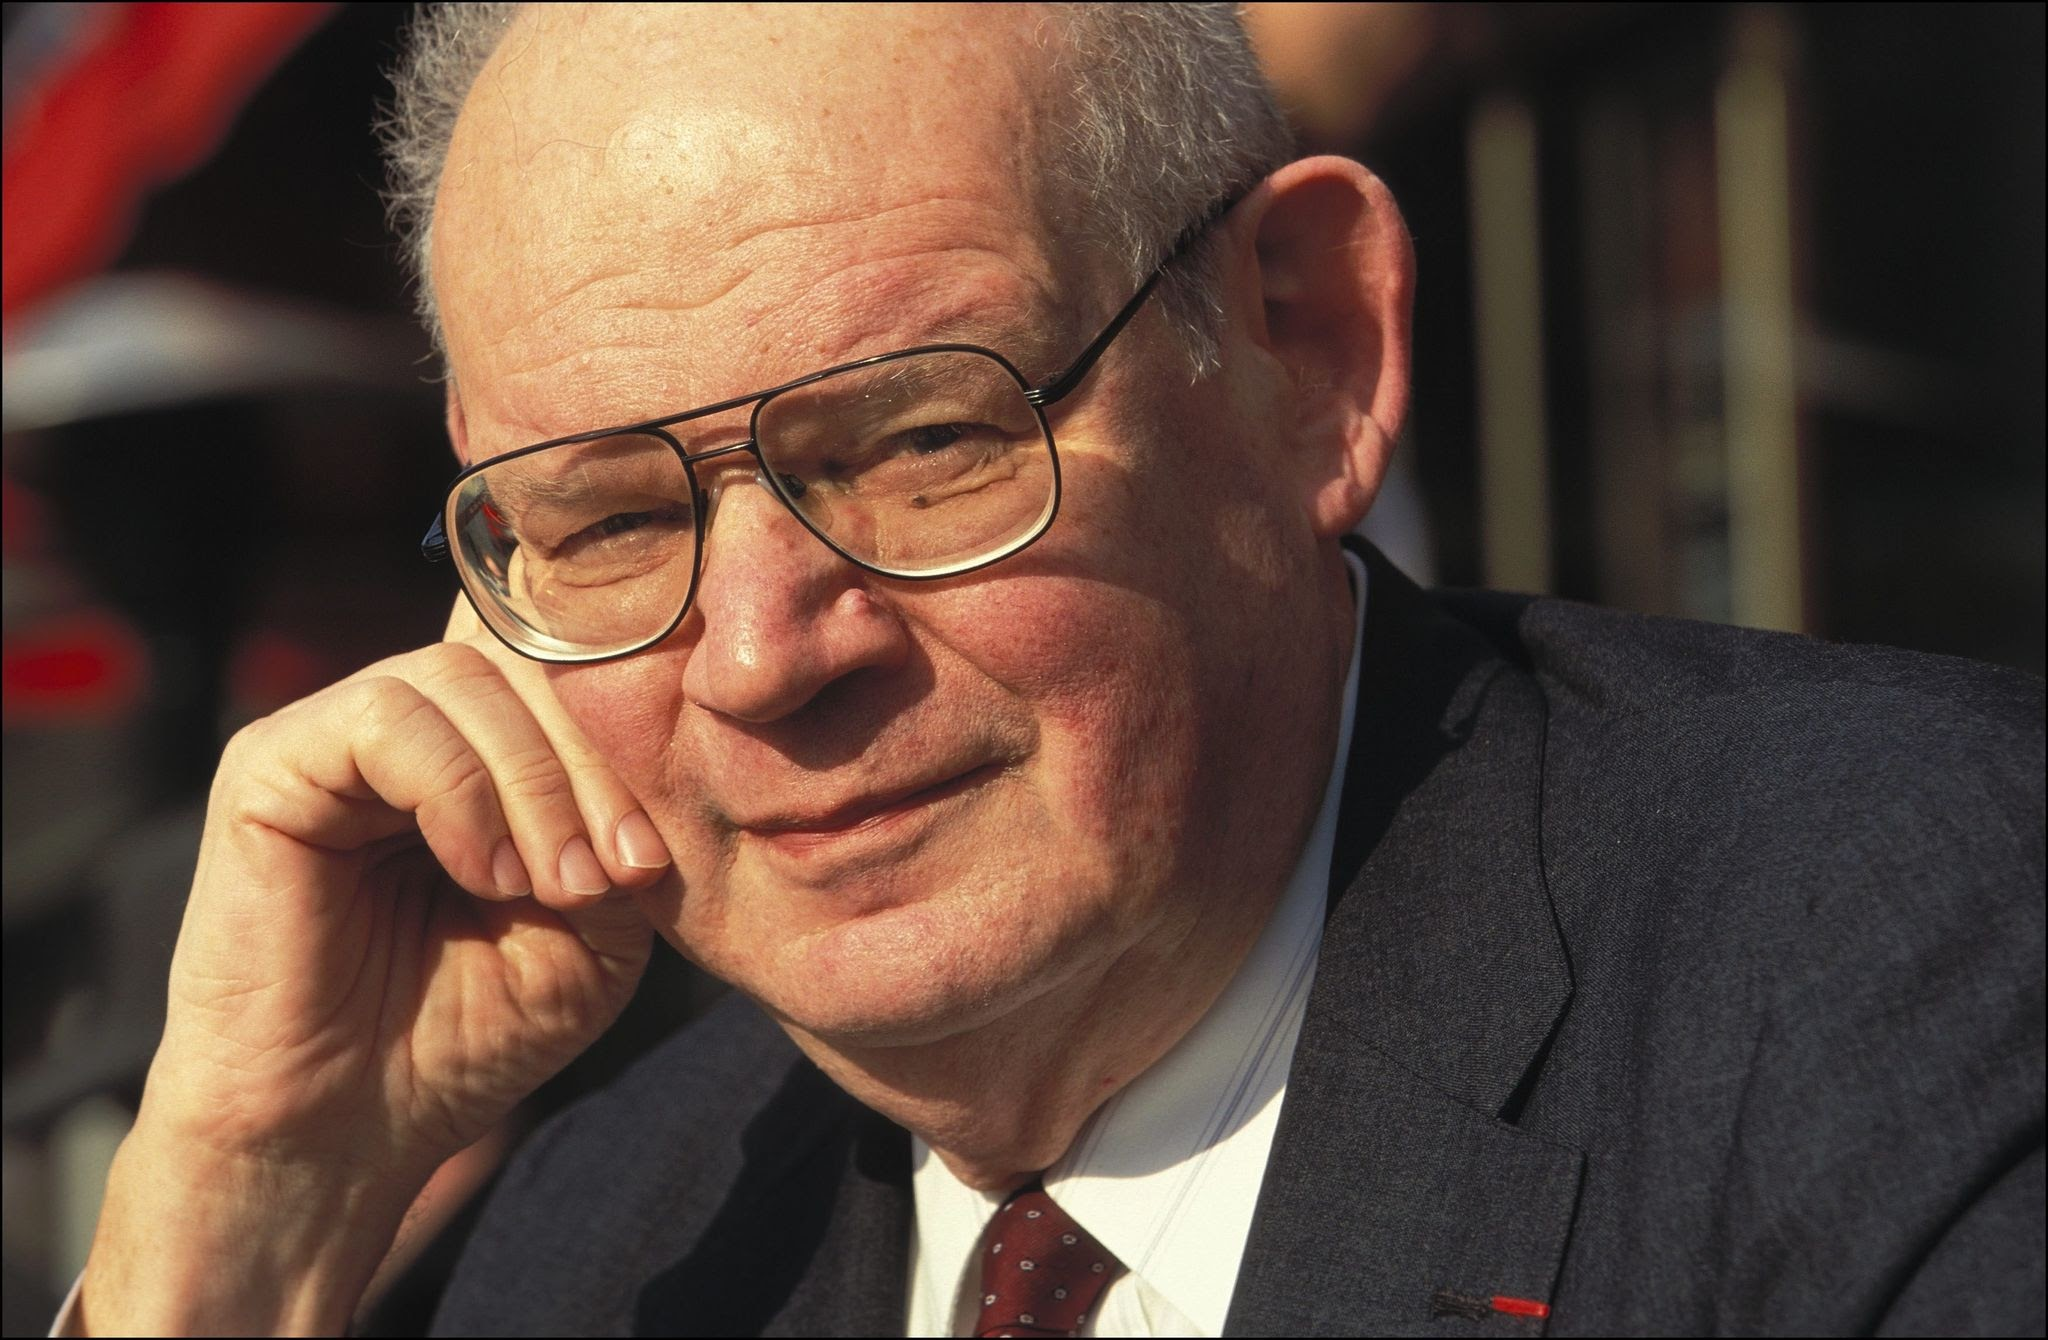
\includegraphics[width=0.7\textwidth]{images/benoit-mandelbrot}
  \caption{Benoît Mandelbrot 1997 in Frankreich~\cite{gaillarde_benoit_1997}.}
\end{center}
\end{figure}

\noindent\textbf{A.4:}\label{app:4}
\begin{figure}[H]\figuretag{A.4}\label{fig:escape-radius}
  \begin{center}
    \begin{tikzpicture}
      \begin{scope}[thick,font=\scriptsize]
        \fill[draw=black, fill=white] (0,0) circle (2);

        \draw [fill=black] (1,1.6) circle(0.05);
        \draw [fill=black] (-3,2.75) circle(0.05);
        \node at (1.75,1.85) {$ P_1(1|1.6i)$};
        \node at (-1.75,3) {$ P_2(-3|2.75i)$};

        \draw [->] (-4,0) -- (4,0) node [above left]  {$Re$};
        \draw [->] (0,-4) -- (0,4) node [below right] {$Im$};

        \foreach \n in {-3,...,-1,1,2,...,3}{
          \draw (\n, 3pt) -- (\n, -3pt)   node [below] {$\n$};
          \draw (3pt,\n) -- (-3pt,\n)   node [left] {$\n i$};
        }
      \end{scope}
    \end{tikzpicture}
    \caption{
      Einheitskreis mit dem Radius 2. Zu sehen ist der Punkt $P_1$, der im
      Einheitskreis liegt und Punkt $P_2$, der außerhalb des Einheitskreises liegt.
    }
  \end{center}
\end{figure}

\noindent\textbf{A.5:}\label{app:5}
\begin{figure}[H]\figuretag{A.5}\label{fig:body-and-head-of-mandelbrot-set}
\begin{center}
  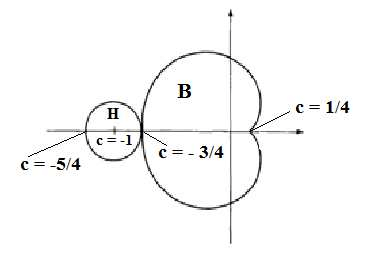
\includegraphics[width=0.7\textwidth]{images/bodyHeadMandelbrotSet}
  \caption{
    K\"orper (B) und Kopf (H) der Mandelbrot-Menge~\cite{mahanta_mandelbrot_2016}.
  }
\end{center}
\end{figure}

\noindent\textbf{A.6:}\label{app:6}
\begin{figure}[H]\figuretag{A.6}\label{fig:mandelbrot-set-zoom-images}
  \centering
  \begin{minipage}[t]{0.40\textwidth}
    \centering
    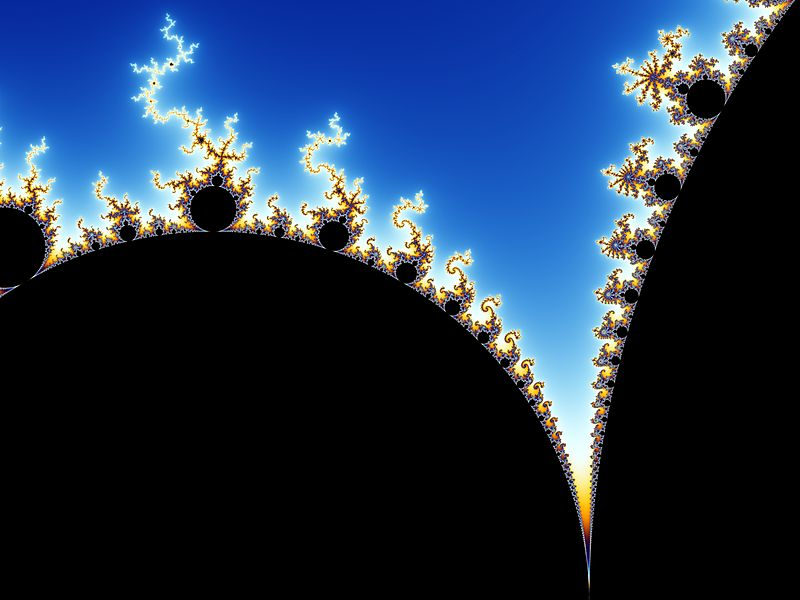
\includegraphics[width=\linewidth]{images/zoom/800px-Mandel_zoom_01_head_and_shoulder}
    \figuretag{A.6.1}
    \vspace*{-4ex}
    \caption{Spalte zwischen Kopf und K\"orper~\cite{beyer_partial_2005}}
    \label{app:6.1}
  \end{minipage}%
  \hspace{8ex}
  \begin{minipage}[t]{0.40\textwidth}
    \centering
    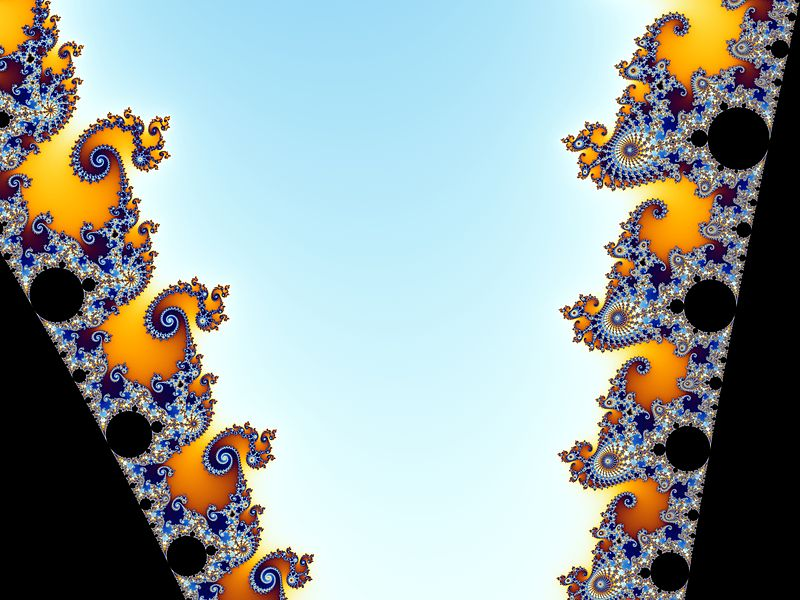
\includegraphics[width=\linewidth]{images/zoom/800px-Mandel_zoom_02_seehorse_valley}
    \figuretag{A.6.2}
    \vspace*{-4ex}
    \caption{\grqq Tal der Seepferdchen\glqq~\cite{beyer_partial_2005-1}}
    \label{app:6.2}
  \end{minipage}
  \\[4ex]
  \begin{minipage}[t]{0.40\textwidth}
    \centering
    
\includegraphics[width=\linewidth]{images/zoom/800px-Mandel_zoom_03_seehorse}
    \figuretag{A.6.3}
    \vspace*{-4ex}
    \caption{Rechts ein deformierter Satellit und links Misiurewicz-Punkt~\cite{beyer_partial_2005-2}}
    \label{app:6.3}
  \end{minipage}%
  \hspace{8ex}
  \begin{minipage}[t]{0.40\textwidth}
    \centering
    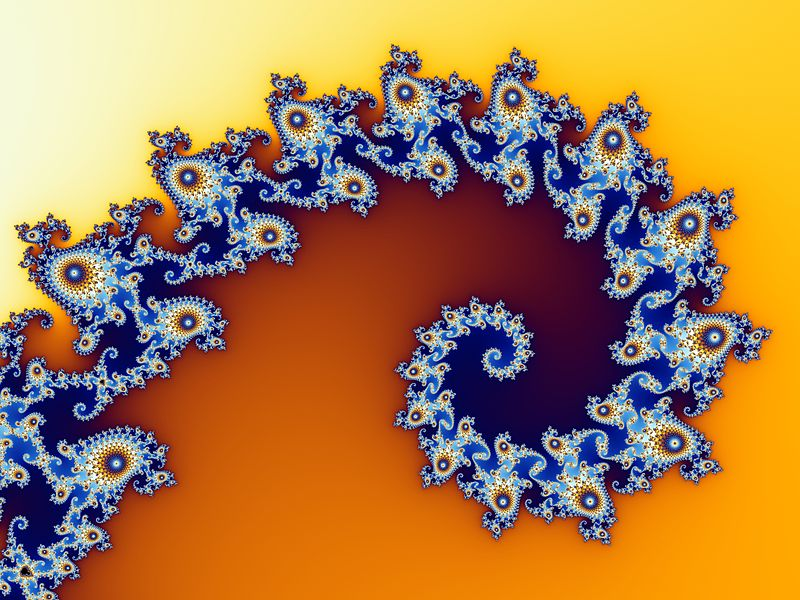
\includegraphics[width=\linewidth]{images/zoom/800px-Mandel_zoom_04_seehorse_tail}
    \figuretag{A.6.4}
    \vspace*{-4ex}
    \caption{Misiurewicz-Punkt~\cite{beyer_partial_2005-3}}
    \label{app:6.4}
  \end{minipage}
  \\[4ex]
  \begin{minipage}[t]{\textwidth}
    \centering
    
\includegraphics[width=0.45\linewidth]{images/zoom/800px-Mandel_zoom_08_satellite_antenna}
    \figuretag{A.6.5}
    \vspace*{-2ex}
    \caption{Satellit mit ähnlicher Struktur wie das Apfelm\"annchen~\cite{beyer_partial_2005-4}}
    \label{app:6.5}
  \end{minipage}
\end{figure}

\end{document}